\section{Program gto\char`_genomic\char`_period}
The \texttt{gto\char`_genomic\char`_period} calculates the best order depth of a sequence, using FCMs. It only works "ACGT", while the rest will be discarded.\\
This application has a dependency to represent the results. It requires the Gnuplot to show the execution result.\\
For help type:
\begin{lstlisting}
./gto_genomic_period -h
\end{lstlisting}
In the following subsections, we explain the input and output paramters.

\subsection*{Input parameters}

The \texttt{gto\char`_genomic\char`_period} program needs program needs two streams for the computation, namely the input and output standard. The input stream is a sequence file.\\
The attribution is given according to:
\begin{lstlisting}
Usage: ./gto_genomic_period [options] [[--] args]
   or: ./gto_genomic_period [options]

It calculates the best order depth of a sequence, using FCMs.It only works "ACGT", 
while the rest will be discarded.

    -h, --help        show this help message and exit

Basic options
    < input.seq       Input sequence file format (stdin)
    > output          Output is given by log_2(4)*K(x)/|x|) (stdout)

Example: ./gto_genomic_period < input.seq > output
\end{lstlisting}
An example of such an input file is:
\begin{lstlisting}
TCTTTACTCGCGCGTTGGAGAAATACAATAGTGCGGCTCTGTCTCCTTATGAAGTCAACAATTTCGCTGGGACTTGCGGC
TCTTTACTCGCGCGTTGGAGAAATACAATAGTGCGGCTCTGTCTCCTTATGAAGTCAACAATTTCGCTGGGACTTGCGGC
GACTTCATCGTGGTCTCTGTCATTATGCGCTCCAACGCATAACTTTGCGCCAGAAGATAGATAGAATGGTGTAAGAAACT
GTAATATATATAATGAACTTCGGCGAGTCTGTGGAGTTTTTGTTGCATTAGAGAGCCAAGAGGTCGGACGTCCTCACGTA
GCCCGAGACGGGCAGGGCGATGGCGACTGAACGGGCTCCATATCACTTTGAGCTTTTATGCTTTCGACTCCTCCAGGAGC
TGAACAACCTTGTTCCCGGCAAAGCCCACTGCGTCATGGAGCTCACGGTCTACATTCATGACTGACTAACCGTAAACTGC
\end{lstlisting}

\subsection*{Output}
The output of the \texttt{gto\char`_genomic\char`_period} program is a execution report, followed by the plot with this information.\\
Using the input above, an report example for this is the following:
\begin{lstlisting}
Running order: 1 ... Done!
Running order: 2 ... Done!
Running order: 3 ... Done!
Running order: 4 ... Done!
Running order: 5 ... Done!
Running order: 6 ... Done!
Running order: 7 ... Done!
Running order: 8 ... Done!
Running order: 9 ... Done!
Running order: 10 ... Done!
Running order: 11 ... Done!
Running order: 12 ... Done!
Running order: 13 ... Done!
Running order: 14 ... Done!
Running order: 15 ... Done!
Running order: 16 ... Done!
Running order: 17 ... Done!
Running order: 18 ... Done!
Running order: 19 ... Done!
Running order: 20 ... Done!
 1	2.246
 2	2.225
 3	2.237
 4	2.079
 5	1.821
 6	1.733
 7	1.717
 8	1.708
 9	1.717
10	1.712
11	1.717
12	1.721
13	1.725
14	1.729
15	1.733
16	1.738
17	1.742
18	1.746
19	1.75
20	1.754
\end{lstlisting}

In the Figure~\ref{fig:gtoGenomicPeriod} is represented the plot for the execution above.

 \begin{figure}[!h]
  \centering
  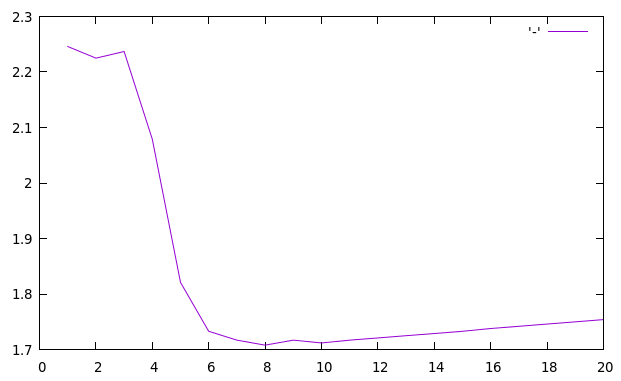
\includegraphics[scale=0.7]{./images/gto_genomic_period.png}
  \caption{\texttt{gto\char`_genomic\char`_period} execution plot.}
  \label{fig:gtoGenomicPeriod}
 \end{figure}